\section{Exploración con sujetos controles}
\subsection{Demográficos}

En la tabla \ref{tab:demHC} se muestran las medidas demográficas de los pacientes dependientes a cocaína y la submuestra independiente de controles.
No hubo diferencia significativa en el sexo ni nivel educativo; los sujetos con dependencia fueron significativamente mayores y con una mayor proporción de fumadores que los controles.

\begin{table}[hbp]
    \centering
    \small
    \caption{Datos demográficos entre pacientes con adicción y controles}
    \label{tab:demHC}
    \begin{tabular}{lccc}
        \hline
        & Con adicción & Controles & \multirow{2}{*}{p}\\
        & (N=46) & (N=45) & \\
        \hline
        Sexo            &  &  & 0.737\\
        - M           & 40 (87.0\%) & 37 (82.2\%) & \\
        - F           & 6 (13.0\%) & 8 (17.8\%) & \\
        Edad            & 34.5 ±  7.9 & 30.5 ±  7.5 & 0.016\\
        Educación       & 13.1 ±  3.0 & 12.8 ±  3.5 & 0.747\\
        Fumar           &  &  & 0.002\\
        - No          & 10 (22.2\%) & 25 (56.8\%) & \\
        - Sí          & 35 (77.8\%) & 19 (43.2\%) & \\
        Cigarrillos al día &  6.6 ± 10.5 &  0.5 ±  0.8 & 0.000\\
        \hline
    \end{tabular}
\end{table}

\subsection{Topología de red}
Se exploraron las medidas topológicas a lo largo de los distintos umbrales.
Para esta comparación se reportan los resultados hasta $\tau = 0.35$, ya que posterior a este las redes de los sujetos controles comenzaron a mostrar desconexión.\par
Los pacientes con adicción tuvieron un mayor número de conexiones y mayor fuerza en las mismas en comparación con las redes de sujetos controles
bajo el mismo umbral (Figura \ref{fig:dsHC}).

\begin{figure}[!ht]
    \centering
    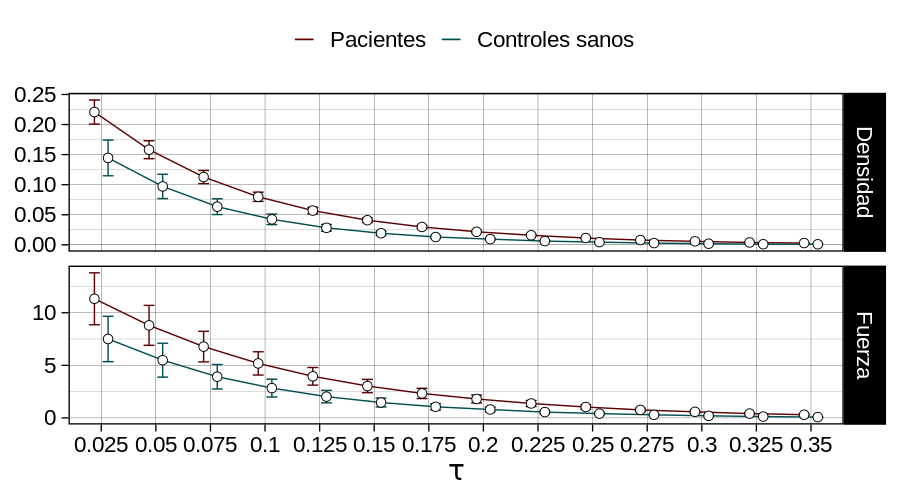
\includegraphics[width=0.8\textwidth]{dens_str_VS.png}
    \caption{Medidas de densidad y fuerza de redes de conectividad  de los pacientes con adicción y controles bajo los distintos umbrales (valores de $\tau$)}
    \label{fig:dsHC}
\end{figure}

De manera similar, los pacientes con adicción mostraron, a su vez, una mayor eficiencia tanto a nivel local como a nivel global que sus pares controles en todos los umbrales explorados (Figura \ref{fig:effHC}).

\begin{figure}[!ht]
    \centering
    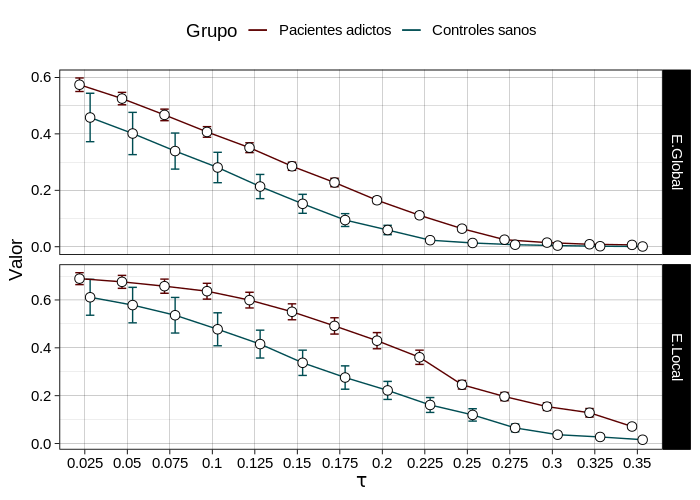
\includegraphics[width=0.8\textwidth]{effs_VS.png}
    \caption{Medidas de eficiencia local y global de redes de conectividad de pacientes con adicción y controles bajo distintos umbrales (valores de $\tau$)}
    \label{fig:effHC}
\end{figure}

No obstante, los pacientes con adicción obtuvieron una menor métrica de mundo pequeño.
En los umbrales más permisivos la diferencia es mínima, pero conforme disminuye la densidad de la red la cualidad de mundo pequeño de las redes de controles sanos aumenta en mayor medida que la de los pacientes dependientes (Figura \ref{fig:sigmaHC}).

\begin{figure}[!ht]
    \centering
    \begin{subfigure}[t]{0.8\textwidth}
        \centering
        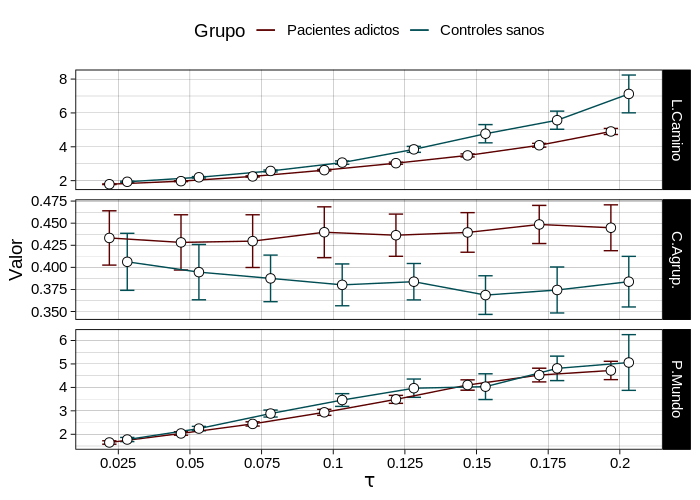
\includegraphics[width=\textwidth]{sigma1_VS.png}
        \caption{Umbrales bajos}
        \label{fig:sigma1}
    \end{subfigure}
    \begin{subfigure}[t]{0.8\textwidth}
        \centering
        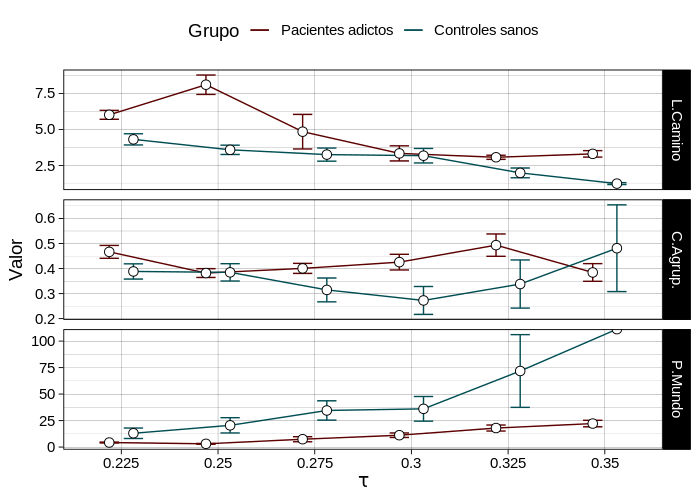
\includegraphics[width=\textwidth]{sigma2_VS.png}
        \caption{Umbrales altos}
        \label{fig:sigma2}
    \end{subfigure}
    \caption{Longitud de camino, coeficiente de agrupamiento y métrica de mundo pequeño en redes de conectividad de pacientes con adicción y controles bajo distintos umbrales (niveles de $\tau$)}
    \label{fig:sigmaHC}
\end{figure}

Tomando un valor de $\tau$ intermedio de 0.25, en la tabla \ref{tab:lmHC} se enlistan las regresiones lineares multivariadas de las distintas métricas de grafo comparando las redes de los pacientes dependientes contra aquellas de controles y tomando edad, sexo y nivel educativo como covariantes. El grupo experimental fue un predictor significativo para todas las variables dependientes.

% Table created by stargazer v.5.2.2 by Marek Hlavac, Harvard University. E-mail: hlavac at fas.harvard.edu
% Date and time: Mon, Sep 16, 2019 - 09:43:43 PM
\begin{table}[!htbp] \centering
  \caption{Regresiones lineales múltiples de métricas de topología de red incluyendo sexo, edad y educación como covariantes}
  \label{tab:lmHC}
  \small
\begin{tabular}{@{\extracolsep{5pt}}lccccc}
\\[-1.8ex]\hline
\hline \\[-1.8ex]
 & \multicolumn{5}{c}{Variables dependientes} \\
\cline{2-6}
\\[-1.8ex] & Densidad & Fuerza & E.Global & E.Local & MundoP. \\
\\[-1.8ex] & (1) & (2) & (3) & (4) & (5)\\
\hline \\[-1.8ex]
 Grupo(HC) & $-$0.007$^{***}$ & $-$0.626$^{***}$ & $-$0.051$^{***}$ & $-$0.126$^{***}$ & 17.766$^{***}$ \\
  & (0.0002) & (0.036) & (0.002) & (0.005) & (1.094) \\
  Sexo(F) & $-$0.0004$^{*}$ & $-$0.113$^{**}$ & $-$0.001 & $-$0.009 & $-$0.485 \\
  & (0.0002) & (0.049) & (0.002) & (0.006) & (1.479) \\
  Edad & $-$0.00000 & $-$0.003 & $-$0.0001 & $-$0.0001 & 0.091 \\
  & (0.00001) & (0.002) & (0.0001) & (0.0003) & (0.071) \\
  Educación & 0.0001$^{**}$ & 0.010$^{*}$ & 0.0003 & 0.001$^{*}$ & $-$0.300$^{*}$ \\
  & (0.00003) & (0.005) & (0.0002) & (0.001) & (0.166) \\
  Constant & 0.011$^{***}$ & 1.009$^{***}$ & 0.063$^{***}$ & 0.234$^{***}$ & 3.914 \\
  & (0.0005) & (0.100) & (0.004) & (0.013) & (3.039) \\
 \hline \\[-1.8ex]
Observaciones & 91 & 91 & 91 & 91 & 91 \\
R$^{2}$ & 0.953 & 0.794 & 0.927 & 0.898 & 0.764 \\
R$^{2} ajustada$ & 0.950 & 0.784 & 0.924 & 0.893 & 0.753 \\
SE Residual (df = 86) & 0.001 & 0.166 & 0.007 & 0.022 & 5.033 \\
F (df = 4; 86) & 432.703$^{***}$ & 82.777$^{***}$ & 273.509$^{***}$ & 188.366$^{***}$ & 69.479$^{***}$ \\
\hline
\hline \\[-1.8ex]
\textit{Nota:}  & \multicolumn{5}{r}{$^{*}$p$<$0.1; $^{**}$p$<$0.05; $^{***}$p$<$0.01} \\
\end{tabular}
\end{table}

\section{Fase cerrada (Doble-ciego)}
\subsection{Clínica}

\begin{table}[!ht]
    \small
    \caption{Medidas demográficas y clínicas de la fase cerrada del proyecto}
    \label{tab:demT}
    \centering
    \begin{tabular}{lccccc}
        \hline
 & \multicolumn{2}{c}{Pre}  &  &\multicolumn{2}{c}{Post} \\
 \cline{2-4}\cline{5-6}
 & Sham & Real & & Sham & Real\\
 & (N=18) & (N=22) &  & (N=18) & (N=22) \\
 \hline
        Sexo            &  &  & &  &  \\
        - M           & 16 (88.89\%) & 19 (86.36\%) &  & 16 (88.89\%) & 19 (86.36\%) \\
        - F           & 2 (11.11\%) & 3 (13.64\%) &  & 2 (11.11\%) & 3 (13.64\%) \\
        Edad            & 33.11 ± 9.13 & 35.32 ± 7.13  &  & 33.11 ± 9.13 & 35.32 ± 7.13 \\
        Educación       & 12.92 ± 2.78 & 13.18 ± 3.08  &  & 12.92 ± 2.78 & 13.18 ± 3.08 \\
        Años de consumo    & 10.19 ± 8.27 & 11.59 ± 8.15  &  & 10.19 ± 8.27 & 11.59 ± 8.15 \\
        Tabaco          &  &   &  &  &   \\
        - No          & 3 (16.67\%) & 6 (27.27\%)  &  & 3 (16.67\%) & 6 (27.27\%)  \\
        - Sí          & 15 (83.33\%) & 16 (72.73\%)  &  & 15 (83.33\%) & 16 (72.73\%) \\
        Cigarrillos al día & 4.36 ± 4.23 & 8.70 ± 13.85  &  & 4.36 ± 4.23 & 8.70 ± 13.85 \\
        \hline
        VAS             & 2.65 ± 2.98 & 4.07 ± 3.72 &  & 2.35 ± 2.55 & 1.54 ± 2.48 \\
        CCQG            & 199.11 ± 43.70 & 190.64 ± 48.44  &  & 159.56 ± 52.81 & 147.05 ± 49.08 \\
        CCQN            & 142.17 ± 48.99 & 149.09 ± 48.58  &  & 134.00 ± 46.12 & 116.55 ± 47.47  \\
        BIS11           & 60.44 ± 16.66 & 64.86 ± 17.62 &  & 61.78 ± 20.39 & 53.32 ± 18.14 \\
        \hline
    \end{tabular}
\end{table}

En la tabla \ref{tab:demT} se enlistan las variables demográficas y clínicas estratificadas por grupo y por etapa experimental.\par
En la fase basal encontramos una correlación entre las mediciones de \textit{craving}: modalidades de CCQ ($r=0.64,\ p<0.001$) y CCQ versión ``\textit{Now}'' con la escala visual análoga ($r=0.64,\ p<0.001$) (Figura \ref{fig:corrA}); en la fase post-tratamiento, la correlación fue significativa entre las modalidades de CCQ ($r=0.8,\ p<0.001$) y la escala visual análoga estuvo relacionada con todas las demás mediciones clínicas (CCQ-G, $r=0.67,\ p<0.001$; CCQ-N, $r=0.87,\ p<0.001$; BIS-11, $r=0.35,\ p=0.027$) (Figura \ref{fig:corrB}).

\begin{figure}[!htb]
    \centering
    \begin{subfigure}[t]{0.47\textwidth}
        \centering
        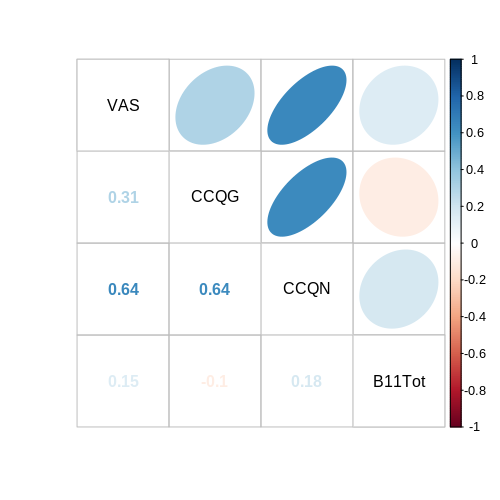
\includegraphics[width=\textwidth]{corr1.png}
        \caption{Fase Pre-tratamiento}
        \label{fig:corrA}
    \end{subfigure}
    \begin{subfigure}[t]{0.47\textwidth}
        \centering
        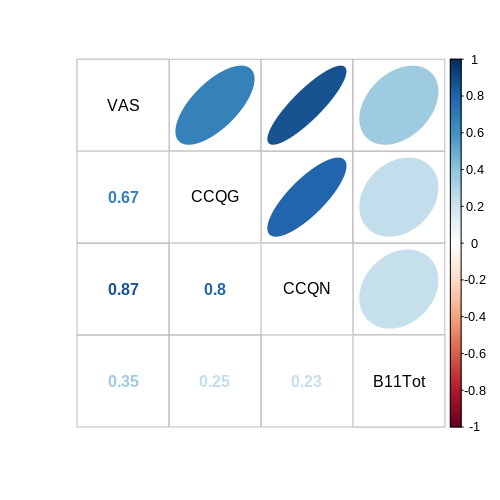
\includegraphics[width=\textwidth]{corr2.png}
        \caption{Fase Post-tratamiento}
        \label{fig:corrB}
    \end{subfigure}
    \caption{Correlación entre las medidas clínicas exploradas en la fase cerrada}
    \label{fig:corrT}
\end{figure}

\begin{figure}[!ht]
    \centering
    \begin{subfigure}[t]{0.475\textwidth}
        \centering
        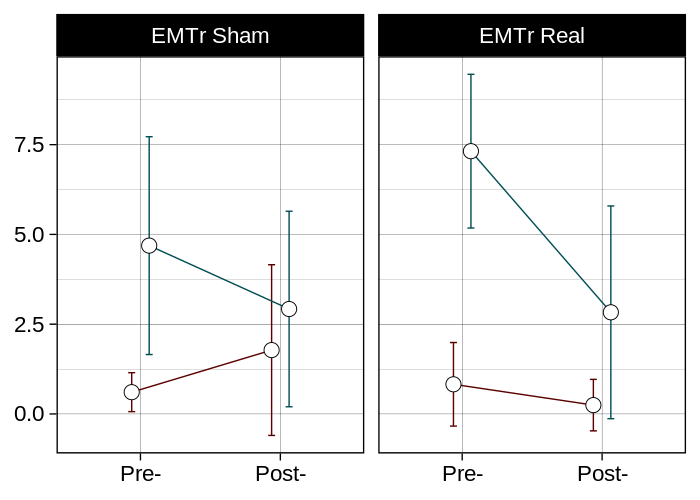
\includegraphics[width=\textwidth]{vasT.png}
        \caption{VAS}
        \label{fig:cl1VAS}
    \end{subfigure}
    \begin{subfigure}[t]{0.475\textwidth}
        \centering
        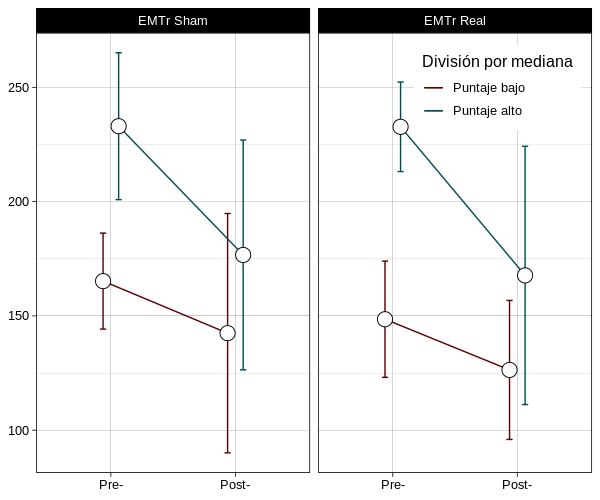
\includegraphics[width=\textwidth]{ccqgT.png}
        \caption{CCQ-G}
        \label{fig:cl1CG}
    \end{subfigure}
    \vskip\baselineskip
    \begin{subfigure}[t]{0.475\textwidth}
        \centering
        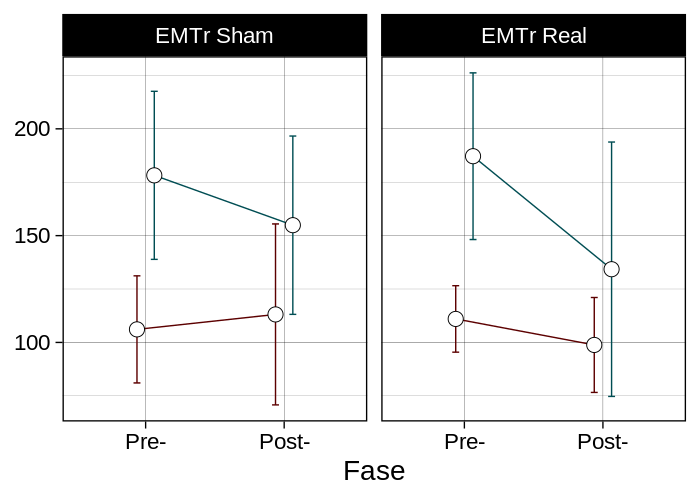
\includegraphics[width=\textwidth]{ccqnT.png}
        \caption{CCQ-N}
        \label{fig:cl1CN}
    \end{subfigure}
    \begin{subfigure}[t]{0.475\textwidth}
        \centering
        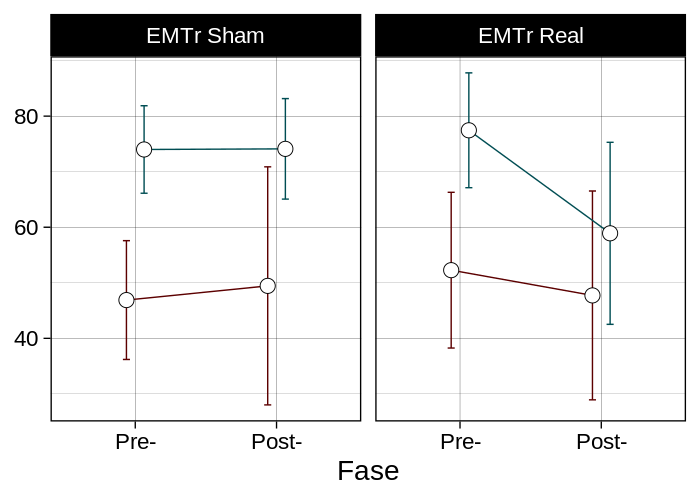
\includegraphics[width=\textwidth]{b11T.png}
        \caption{BIS-11}
        \label{fig:cl1B11}
    \end{subfigure}
    \caption{Correlación entre las medidas clínicas exploradas en ambas mediciones de la fase cerrada del proyecto}
    \label{fig:clin1}
\end{figure}

En las distintas mediciones clínicas se pudo observar un patrón de cambio distinto en los sujetos que mostraban un puntaje basal alto o bajo (separado por la mediana) (Figura \ref{fig:clin1}). Mientras que todos los sujetos que comenzaban con un puntaje alto demostraban una disminución en su puntaje a las dos semanas de tratamiento independientemente del grupo experimental (con excepción de la escala de impulsividad de Barratt, donde el grupo de estimulación sham se mantuvo constante; Figura \ref{fig:cl1B11}), las diferencias entre los grupos de estimulación, cuando hubo, se encontraron principalmente en aquellos sujetos que tuvieron un puntaje basal bajo. \par
En la escala visual análoga, los sujetos de puntaje basal bajo que llevaron estimulación sham expresaron un aumento en el nivel de \textit{craving}, a diferencia de quienes llevaron estimulación real (Figura \ref{fig:cl1VAS}) En menor medida, ocurrió lo mismo con las escalas de CCQ-N (Figura \ref{fig:cl1CN}) y de impulsividad de Barratt (Figura \ref{fig:cl1B11}). En la escala de CCQ-G no hubo diferencia entre grupo experimental ni de puntaje. \par

Debido a estas diferencias se pretendió predecir los puntajes clínicos post-tratamiento utilizando el grupo de tratamiento y los puntajes basales como covariantes\footnote{Debido a la correlación de variables de \textit{craving} basales, para evitar colinealidad solo se introdujo la misma variable basal de esta sintomatología como covariante para cada modelo.}. En la tabla \ref{tab:lmCl1} se muestran los coeficientes y parámetros de los distintos modelos. \par
En todos los modelos, el puntaje basal de la misma escala fue un predictor significativo (VAS, $0.382\ (0.098),\ p<0.01$; CCQ-G, $0.567\ (0.148),\ p<0.01$; CCQ-N, $0.536\ (0.127),\ p<0.01$; BIS-11, $0.876\ (0.127),\ p<0.01$). El grupo experimental fue un predictor significativo en los modelos clínicos de \textit{craving} por medio de la escala visual análoga ($-1.529\ (0.667),\ p<0.05$) y de impulsividad ($-11.335\ (4.242),\ p<0.05$) controlando por el puntaje basal tanto de \textit{craving} como de impulsividad en ambos modelos.

% Table created by stargazer v.5.2.2 by Marek Hlavac, Harvard University. Ebel{}
% Date and time: Tue, Sep 17, 2019 - 12:57:16 AM
\begin{table}[!ht] \centering
  \small
  \caption{Regresiones lineales multivariadas de mediciones clínicas con grupo de tratamiento como predictor y mediciones basales como covariantes}
  \label{tab:lmCl1}
\begin{tabular}{@{\extracolsep{5pt}}lcccc}
\\[-1.8ex]\hline
\hline \\[-1.8ex]
 & \multicolumn{4}{c}{Mediciones clínicas (Post-tratamiento)} \\
\cline{2-5}
\\[-1.8ex] & VAS & CCQ-G & CCQ-N & BIS-11 \\
\\[-1.8ex] & (1) & (2) & (3) & (4)\\
\hline \\[-1.8ex]
 Grupo(Real) & $-$1.529$^{**}$ & $-$11.915 & $-$23.553$^{*}$ & $-$11.335$^{**}$ \\
  & (0.667) & (13.587) & (12.088) & (4.242) \\
  VAS & 0.382$^{***}$ &  &  & $-$0.467 \\
  & (0.098) &  &  & (0.806) \\
  CCQ-G &  & 0.567$^{***}$ &  & 0.003 \\
  &  & (0.148) &  & (0.062) \\
  CCQ-N &  &  & 0.536$^{***}$ & $-$0.044 \\
  &  &  & (0.127) & (0.072) \\
  B11 & 0.039$^{*}$ & 0.953$^{**}$ & 0.540 & 0.876$^{***}$ \\
  & (0.019) & (0.400) & (0.361) & (0.127) \\
  Constant & $-$1.014 & $-$11.005 & 25.146 & 15.610 \\
  & (1.265) & (40.936) & (27.318) & (12.764) \\
 \hline \\[-1.8ex]
Observaciones & 40 & 40 & 40 & 40 \\
R$^{2}$ & 0.391 & 0.355 & 0.409 & 0.619 \\
R$^{2}$ ajustada & 0.341 & 0.301 & 0.360 & 0.563 \\
SE Residual & 2.042  & 42.247  & 37.664  & 12.827  \\
            & (df = 36) &(df = 36)&(df = 36)&(df = 34) \\
Estadístico F & 7.714$^{***}$  & 6.592$^{***}$  & 8.321$^{***}$  & 11.048$^{***}$  \\
              &(df = 3; 36)&(df = 3; 36)&(df = 3; 36)&(df = 5; 34)\\
\hline
\hline \\[-1.8ex]
\textit{Nota:}  & \multicolumn{4}{r}{$^{*}$p$<$0.1; $^{**}$p$<$0.05; $^{***}$p$<$0.01} \\
\end{tabular}
\end{table}

\subsection{Topología de redes}
Tomando la medida de $\tau = 0.25$ exploramos los cambios en la topología de las redes de los distintos grupos experimentales antes y después de las dos semanas de estimulación magnética.\par
Como se observa en la figura \ref{fig:gpT1}, mientras que los sujetos que llevaron dos semanas de estimulación sham obtuvieron un ligero incremento en la densidad y fuerza de sus conexiones; aquellos que llevaron un tratamiento real mostraron una importante disminución en estas mismas métricas. La interacción entre el grupo de estimulación y la fase de estudio resulta ser un predictor significativo tanto para la medida de densidad ($0.004\ (0.000),\ p<0.01$) como de fuerza ($0.347\ (0.075),\ p<0.01$) (tabla \ref{tab:memT1} (1) y (2)).\par

\begin{figure}[!tb]
    \centering
    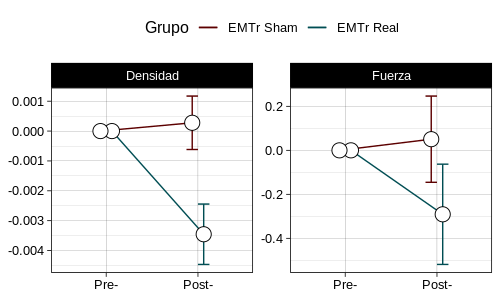
\includegraphics[width=0.7\textwidth]{gphT1.png}
    \caption{Medidas de densidad y fuerza de redes en pacientes con adicción antes y después de dos semanas de tratamiento de EMTr}
    \label{fig:gpT1}
\end{figure}

De forma similar, a las dos semanas de tratamiento encontramos una reducción en las métricas de eficiencia (Figura \ref{fig:gpT2}); mientras que la reducción en la eficiencia local ocurrió igualmente tanto en aquellos sujetos que llevaron estimulación real como en quienes llevaron sham, la eficiencia global disminuyó únicamente en quienes llevaron un tratamiento real. Esto fue confirmado en el modelo de efectos mixtos, donde la interacción del grupo experimental y la fase de tratamiento fue un predictor significativo únicamente para la modalidad global de eficiencia ($-0.042\ (0.003),\ p<0.01$) y no la local ($-0.002\ (0.008),\ p>0.05$) (tabla \ref{tab:memT2} (4) y (3)).\par

\begin{figure}[!htb]
    \centering
    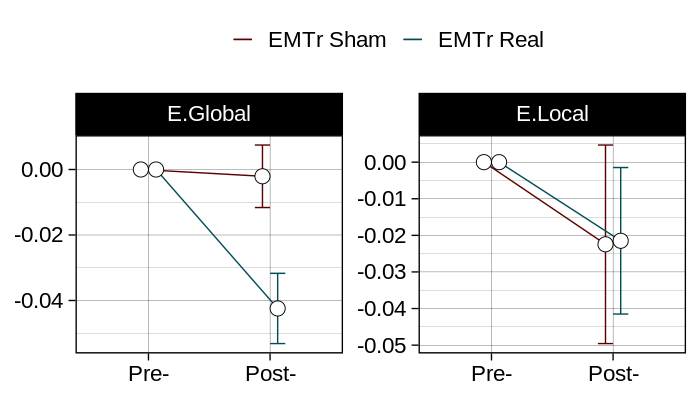
\includegraphics[width=0.7\textwidth]{gphT2.png}
    \caption{Medidas de eficiencia global y local de redes en pacientes con adicción antes y después de dos semanas de tratamiento de EMTr}
    \label{fig:gpT2}
\end{figure}

% Table created by stargazer v.5.2.2 by Marek Hlavac, Harvard University. E-mail: hlavac at fas.harvard.edu
% Date and time: Tue, Sep 17, 2019 - 03:17:17 AM
\begin{table}[!htb] \centering
  \small
  \caption{Modelos de efectos mixtos de medidas de topología de red en fase cerrada del tratamiento de EMTr, con sexo, edad y educación como covariantes}
  \label{tab:memT1}
\begin{tabular}{@{\extracolsep{5pt}}lcccc}
\\[-1.8ex]\hline
\hline \\[-1.8ex]
 & \multicolumn{4}{c}{Variables dependientes} \\
\cline{2-5}
\\[-1.8ex] & Densidad & Fuerza & E.Local & E.Global \\
\\[-1.8ex] & (1) & (2) & (3) & (4)\\
\hline \\[-1.8ex]
 Fase(Post-) & 0.0003 & 0.049 & $-$0.023$^{***}$ & $-$0.002 \\
  & (0.0002) & (0.051) & (0.005) & (0.002) \\
  Grupo(Real) & 0.004$^{***}$ & 0.373$^{***}$ & 0.036$^{***}$ & 0.034$^{***}$ \\
  & (0.0004) & (0.094) & (0.009) & (0.004) \\
  VAS & $-$0.00004 & $-$0.005 & $-$0.001 & $-$0.0003 \\
  & (0.00005) & (0.010) & (0.001) & (0.0005) \\
  B11 & $-$0.00001 & 0.0005 & 0.00003 & $-$0.0001 \\
  & (0.00001) & (0.002) & (0.0002) & (0.0001) \\
  Sexo(F) & 0.0001 & $-$0.081 & $-$0.0004 & $-$0.002 \\
  & (0.001) & (0.130) & (0.013) & (0.005) \\
  Edad & $-$0.00003 & $-$0.005 & $-$0.0001 & $-$0.0001 \\
  & (0.00003) & (0.006) & (0.001) & (0.0002) \\
  Educación & 0.0001 & 0.017 & 0.001 & 0.001 \\
  & (0.0001) & (0.016) & (0.002) & (0.001) \\
  Fase:Grupo & $-$0.004$^{***}$ & $-$0.347$^{***}$ & $-$0.002 & $-$0.042$^{***}$ \\
  & (0.0003) & (0.075) & (0.008) & (0.003) \\
  Constante & 0.014$^{***}$ & 1.149$^{***}$ & 0.280$^{***}$ & 0.115$^{***}$ \\
  & (0.001) & (0.289) & (0.029) & (0.012) \\
 \hline \\[-1.8ex]
Observaciones & 80 & 80 & 80 & 80 \\
Crit. I. Akaike & $-$704.206 & 62.957 & $-$260.588 & $-$380.011 \\
Crit. I. Bayesiano & $-$678.003 & 89.159 & $-$234.386 & $-$353.809 \\
\hline
\hline \\[-1.8ex]
\textit{Nota:}  & \multicolumn{4}{r}{$^{*}$p$<$0.1; $^{**}$p$<$0.05; $^{***}$p$<$0.01} \\
\end{tabular}
\end{table}

Al evaluar la eficiencia de forma global y en comparación con redes aleatorias equivalentes, encontramos una interacción significativa entre el grupo experimental y la fase de tratamiento para el escalar de mundo pequeño ($1.804\ (0.2),\ p<0.01$) y la longitud de camino característica ($0.935\ (0.185),\ p<0.01$), una de las dos medidas de donde esta se deriva (tabla \ref{tab:memT2}). \par
La longitud de camino característica aumentó en mayor medida en los participantes del grupo de estimulación real que los del grupo placebo. El coeficiente de agrupamiento fue también mayor en este grupo mientras que los participantes que recibieron estimulación sham mostraron una ligera disminución en esta medida. Sin embargo, esta diferencia no resultó significativa en el modelo explorado ($0.013\ (0.009),\ p>0.05$) (tabla \ref{tab:memT2} (2)). \par
En los participantes cuyas dos semanas de tratamiento consistió en estimulación real notamos un incremento en la métrica de mundo pequeño comparada con la calculada a partir de sus redes en la etapa basal al contrario de aquellos participantes donde la estimulación fue sham, en quienes esta métrica disminuyó a las dos semanas del tratamiento (Figura \ref{fig:gpT3}).

\begin{figure}[!htb]
    \centering
    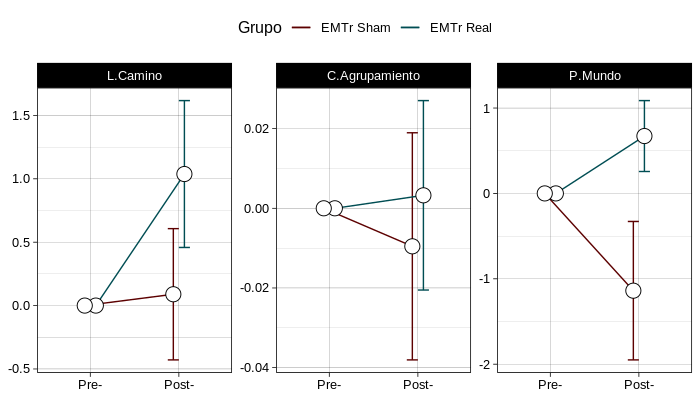
\includegraphics[width=0.9\textwidth]{gphT3.png}
    \caption{Medidas de longitud de camino, coeficiente de agrupamiento y escalar de mundo pequeño de redes de pacientes con adicción antes y después de dos semanas de tratamiento de EMTr}
    \label{fig:gpT3}
\end{figure}

% Table created by stargazer v.5.2.2 by Marek Hlavac, Harvard University. E-mail: hlavac at fas.harvard.edu
% Date and time: Tue, Sep 17, 2019 - 03:28:16 AM
\begin{table}[!htb] \centering
    \small
  \caption{Modelos de efectos mixtos de métricas de mundo pequeño en la fase cerrada de tratamiento con sexo, edad y educación como covariantes}
  \label{tab:memT2}
\begin{tabular}{@{\extracolsep{5pt}}lccc}
\\[-1.8ex]\hline
\hline \\[-1.8ex]
 & \multicolumn{3}{c}{Variables dependientes} \\
\cline{2-4}
\\[-1.8ex] & L.Camino & C.Agrupamiento & MundoP. \\
\\[-1.8ex] & (1) & (2) & (3)\\
\hline \\[-1.8ex]
 Fase(Post-) & 0.079 & $-$0.010$^{*}$ & $-$1.134$^{***}$ \\
  & (0.131) & (0.006) & (0.144) \\
  Grupo(Real) & $-$0.816$^{***}$ & 0.020$^{**}$ & $-$1.075$^{***}$ \\
  & (0.151) & (0.008) & (0.140) \\
  VAS & $-$0.022 & $-$0.001 & 0.008 \\
  & (0.019) & (0.001) & (0.017) \\
  B11 & 0.003 & 0.0001 & $-$0.002 \\
  & (0.003) & (0.0002) & (0.003) \\
  Sexo(F) & $-$0.145 & 0.004 & $-$0.063 \\
  & (0.181) & (0.011) & (0.149) \\
  Edad & 0.011 & $-$0.0002 & 0.014$^{**}$ \\
  & (0.008) & (0.0005) & (0.007) \\
  Educación & $-$0.031 & 0.001 & 0.003 \\
  & (0.023) & (0.001) & (0.019) \\
  Fase:Grupo & 0.935$^{***}$ & 0.012 & 1.804$^{***}$ \\
  & (0.185) & (0.009) & (0.200) \\
  Constante & 6.305$^{***}$ & 0.359$^{***}$ & 4.363$^{***}$ \\
  & (0.442) & (0.025) & (0.375) \\
 \hline \\[-1.8ex]
Observaciones & 80 & 80 & 80 \\
Crit. Inf. Akaike & 155.643 & $-$265.029 & 149.617 \\
Crit. Inf. Bayesiano & 181.845 & $-$238.827 & 175.819 \\
\hline
\hline \\[-1.8ex]
\textit{Nota:}  & \multicolumn{3}{r}{$^{*}$p$<$0.1; $^{**}$p$<$0.05; $^{***}$p$<$0.01} \\
\end{tabular}
\end{table}

\section{Fase abierta (3 meses)}
\subsection{Clínica}
En la tabla \ref{tab:cl2} enlistamos las puntuaciones clínicas de los sujetos que completaron los 3 meses de tratamiento real en su etapa basal (T0), a dos semanas de tratamiento real (T1) y 3 meses de sesiones de mantenimiento (T2).

\begin{table}[!htb]
    \centering
    \small
    \caption{Mediciones clínicas longitudinales (Basales: T0; Tratamiento: T1; Mantenimiento: T2)}
    \label{tab:cl2}
\begin{tabular}{lcccc}
\hline
 & T0 & T1 & T2 & \multirow{2}{*}{p}\\
 & (N=16) & (N=16) & (N=16) &  \\
\hline
VAS   &  3.8 ±  4.0 &  0.9 ±  2.3 &  0.3 ±  0.8 & 0.001\\
CCQ-G  & 200.1 ± 43.1 & 135.4 ± 45.4 & 128.6 ± 49.0 & 0.000\\
CCQ-N  & 156.5 ± 48.5 & 114.6 ± 45.7 & 110.2 ± 29.5 & 0.005\\
BIS-11 & 67.9 ± 14.8 & 54.1 ± 17.1 & 52.2 ± 17.2 & 0.019\\
\hline
\end{tabular}
\end{table}

\textit{Grosso modo} observamos una mayor mejoría clínica en los participantes con puntuaciones basales más altas después de las dos semanas de tratamiento que se mantiene independientemente de la situación basal a los tres meses de tratamiento (Figura \ref{fig:clin2}).\par
Hubo una interacción significativa entre el grupo de puntaje basal y la fase de medición en las mediciones de craving, donde el grupo con un puntaje basal mayor tuvo una mejoría más importante que el grupo de puntaje bajo (tabla \ref{tab:clin2}); esto fue significativo para las dos semanas en la escala visual análoga ($-5.05\ (1.21),\ p<0.01$); y CCQ versión general ($-61.63\ (24.99)\, p<0.05$) y a los tres meses de mantenimiento en las tres mediciones (VAS, $-6.19\ (1.21),\ p<0.01$; CCQ-G, $-70.63\ (24.99),\ p<0.01$; CCQ-N, $-44.88\ (20.9)\, p<0.05$). En cuanto a la medición de impulsividad, el cambio longitudinal controlado por covariantes demográficas y puntaje basal, fue significativo a los tres meses ($-13.13\ (5.62),\ p<0.05$) pero no a las dos semanas ($-9.63\ (5.62),\ p>0.05$).

\begin{figure}[!hbt]
    \centering
    \begin{subfigure}[t]{0.475\textwidth}
        \centering
        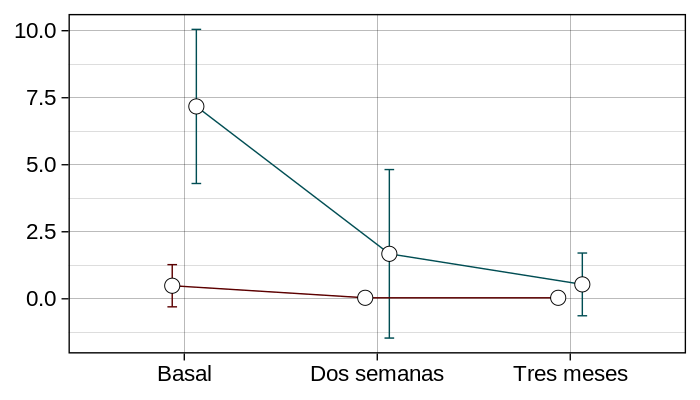
\includegraphics[width=\textwidth]{clinL1.png}
        \caption{VAS}
        \label{fig:cl2VAS}
    \end{subfigure}
    \hfill
    \begin{subfigure}[t]{0.475\textwidth}
        \centering
        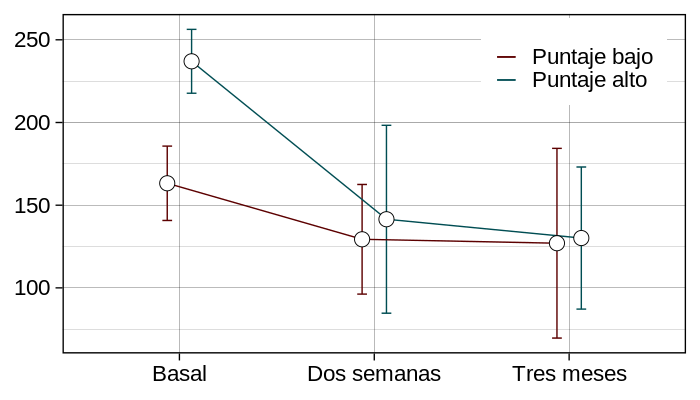
\includegraphics[width=\textwidth]{clinL2.png}
        \caption{CCQ-G}
        \label{fig:cl2CG}
    \end{subfigure}
    \vskip\baselineskip
    \begin{subfigure}[t]{0.475\textwidth}
        \centering
        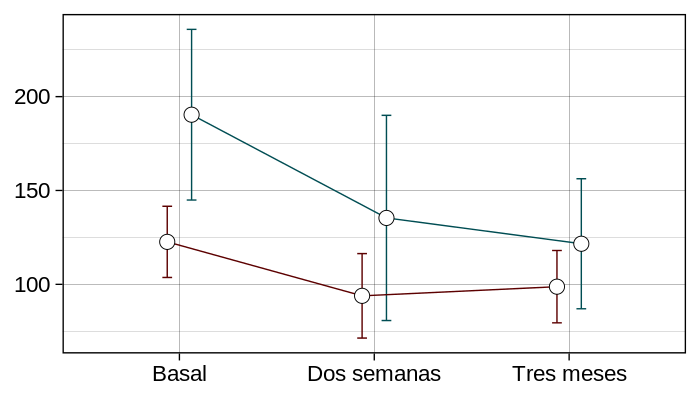
\includegraphics[width=\textwidth]{clinL3.png}
        \caption{CCQ-N}
        \label{fig:cl2CN}
    \end{subfigure}
    \hfill
    \begin{subfigure}[t]{0.475\textwidth}
        \centering
        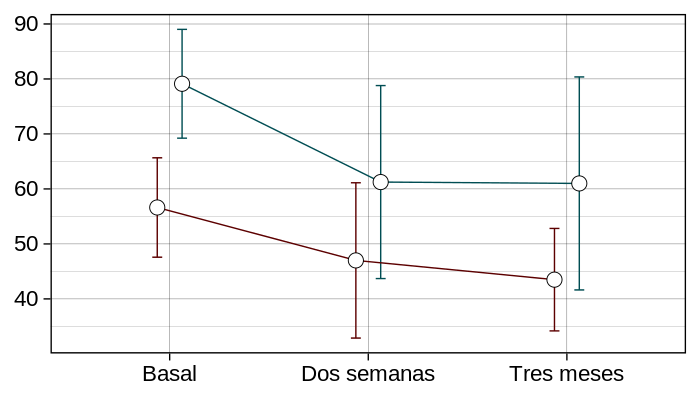
\includegraphics[width=\textwidth]{clinL4.png}
        \caption{BIS-11}
        \label{fig:cl2B11}
    \end{subfigure}
    \caption{Puntajes de mediciones clínicas (basales, tratamiento y mantenimiento) separados por la mediana basal grupal}
    \label{fig:clin2}
\end{figure}

% Table created by stargazer v.5.2.2 by Marek Hlavac, Harvard University. E-mail: hlavac at fas.harvard.edu
% Date and time: Fri, Sep 20, 2019 - 01:04:41 AM
\begin{table}[!htbp] \centering
    \small
    \caption{Modelos de efectos mixtos de las mediciones clínicas longitudinales (hasta tres meses de mantenimiento) incluyendo grupo de puntaje basal y medidas demográficas como covariantes.}
  \label{tab:clin2}
\begin{tabular}{@{\extracolsep{5pt}}lcccc}
\\[-1.8ex]\hline
\hline \\[-1.8ex]
 & \multicolumn{4}{c}{Mediciones clínicas } \\
\cline{2-5}
\\[-1.8ex] & VAS & CCQ-G & CCQ-N & BIS-11\\
\\[-1.8ex] & (1) & (2) & (3) & (4) \\
\hline \\[-1.8ex]
 Fase(T1) & $-$0.450 & $-$33.875$^{*}$ & $-$28.750$^{*}$ & $-$9.625$^{*}$ \\
  & (0.853) & (17.667) & (14.780) & (5.617) \\
  Fase(T2) & $-$0.450 & $-$36.250$^{**}$ & $-$23.875 & $-$13.125$^{**}$ \\
  & (0.853) & (17.667) & (14.780) & (5.617) \\
  Grupo(Mediana) & 6.648$^{***}$ & 83.286$^{***}$ & 66.292$^{***}$ & 21.010$^{***}$ \\
  & (0.858) &  (22.555) &(18.198) & (7.120) \\
  Edad & 0.079$^{**}$ & 1.738 & 1.133 & $-$0.109 \\
  & (0.037) & (1.145) & (0.993) & (0.396) \\
  Sexo(F) & $-$1.105$^{*}$ & $-$19.678 & 7.937 & $-$10.465 \\
  & (0.663) & (19.923) & (17.769) & (6.459) \\
  Educación & $-$0.145$^{*}$ & $-$2.435 & $-$2.665 & $-$1.075 \\
  & (0.087) & (2.915) & (2.291) & (0.836) \\
  FaseT1:GroupMed\textgreater  & $-$5.048$^{***}$ &  $-$61.625$^{**}$  & $-$26.250  & $-$8.250 \\
  & (1.207) & (24.985) & (20.901) & (7.943) \\
  FaseT2:GroupMed\textgreater  & $-$6.188$^{***}$ & $-$70.625$^{***}$  & $-$44.875$^{**}$  & $-$5.000 \\
  & (1.207) & (24.985) & (20.901) & (7.943) \\
  Constante & $-$0.326 & 129.207$^{**}$ & 114.915$^{**}$ & 77.950$^{***}$ \\
  & (1.805) & (52.017) & (46.079) & (16.748) \\
 \hline \\[-1.8ex]
Observaciones & 48 & 48 & 48 & 48 \\
Crit. Inf. Akaike & 202.470 & 446.484 & 434.167 & 357.308 \\
Crit. Inf. Bayesiano & 223.053 & 467.067 & 454.750 & 377.891 \\
\hline
\hline \\[-1.8ex]
\textit{Nota:}  & \multicolumn{4}{r}{$^{*}$p$<$0.1; $^{**}$p$<$0.05; $^{***}$p$<$0.01} \\
\end{tabular}
\end{table}

\FloatBarrier

\subsection{Topología de redes}
Para los análisis longitudinales, se utilizó el mismo nivel de umbral de $\tau$ que los análisis previos y la misma submuestra de los sujetos que completaron los tres meses de mantenimiento. \par
En las métricas topológicas generales de conectividad observamos que el efecto obtenido a las dos semanas de tratamiento se mantiene después de los meses de mantenimiento (Figura \ref{fig:gpL11}). \par
Explorando los modelos de efectos mixtos encontramos que para la densidad de conexiones el coeficiente obtenido a las dos semanas de tratamiento ($-0.007\ (0.001),\ p<0.01$) fue idéntico a los tres meses de mantenimiento ($-0.007\ (0.001),\ p<0.01$). En la fuerza de las conexiones, posterior a la disminución de fuerza a las dos semanas de tratamiento ($-0.75\ (0.1),\ p<0.01$), a los tres meses se encontró también una disminución significativa en comparación con la medición basal ($-0.7\ (0.1),\ p<0.01$) como se refleja en la tabla \ref{tab:memL2}. Aunque hay un ligero aumento entre la medición post-tratamiento y post-mantenimiento (T2\textendash{}T1), en la medición post-hoc esta diferencia no fue significativa ($0.048\ (0.082),\ Z=0.578,\ p>0.83$). Para esta misma medición el modelo arrojó una diferencia significativa entre el sexo, donde las mujeres mostraban una menor fuerza en las conexiones de sus redes que los hombres ($-0.402\ (0.181),\ p<0.05$).

\begin{figure}[!htb]
    \centering
    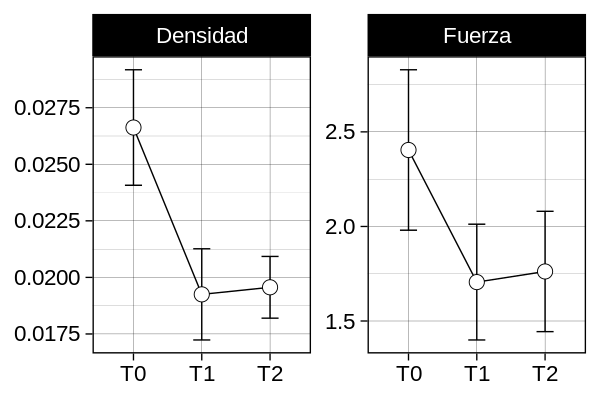
\includegraphics[width=0.7\textwidth]{graphL11.png}
    \caption{Medidas de densidad y fuerza de red de pacientes con adicción en la fase basal (T0), después de dos semanas tratamiento real (T1) y de tres meses de mantenimiento (T2)}
    \label{fig:gpL11}
\end{figure}

En cuanto a la eficiencia, en los modelos encontramos una disminución significativa a las dos semanas de tratamiento en la eficiencia local ($-0.038\ (0.008),\ p<0.001$) y global ($-0.055\ (0.006),\ p<0.01$), que se mantuvo constante después de los tres meses de mantenimiento (eficiencia local, $-0.037\ (0.009),\ p<0.01$; eficiencia global, $-0.056\ (0.007),\ p<0.01$). De la misma forma que la fuerza, encontramos una disminución en la eficiencia local en mujeres en comparación con los hombres ($-0.032\ (0.016),\ p<0.05$). Con la eficiencia global la edad resultó ser una covariante significativa con coeficiente negativo ($-0.002\ (0.001),\ p<0.05$).

\begin{figure}[!htb]
    \centering
    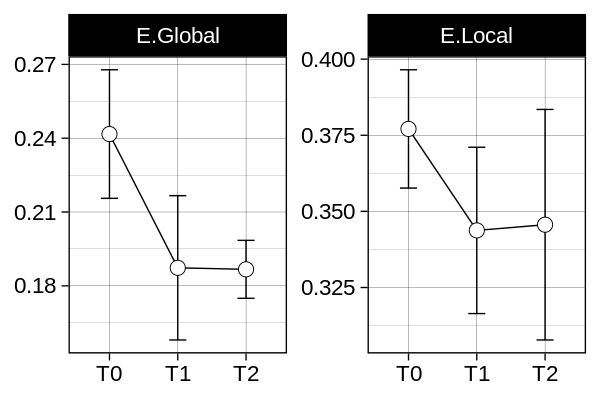
\includegraphics[width=0.7\textwidth]{graphL12.png}
    \caption{Medidas de eficiencia global y local de red en pacientes con adicción en la fase basal (T0), después de dos semanas de tratamiento real (T1) y tres meses de mantenimiento (T2)}
    \label{fig:gpL12}
\end{figure}


% Table created by stargazer v.5.2.2 by Marek Hlavac, Harvard University. E-mail: hlavac at fas.harvard.edu
% Date and time: Fri, Sep 20, 2019 - 03:39:48 AM
\begin{table}[!htbp] \centering
    \small
  \caption{Modelos de efectos mixtos de medidas de topología de red en la fase abierta del proyecto (dos semanas de tratamiento; tres meses de mantenimiento) con medidas demográficas como covariantes}
  \label{tab:memL1}
\begin{tabular}{@{\extracolsep{5pt}}lcccc}
\\[-1.8ex]\hline
\hline \\[-1.8ex]
 & \multicolumn{4}{c}{Variables dependientes} \\
\cline{2-5}
\\[-1.8ex] & Densidad & Fuerza & E.Local & E.Global \\
\\[-1.8ex] & (1) & (2) & (3) & (4)\\
\hline \\[-1.8ex]
 Fase(T1) & $-$0.007$^{***}$ & $-$0.753$^{***}$ & $-$0.038$^{***}$ & $-$0.055$^{***}$ \\
  & (0.001) & (0.101) & (0.008) & (0.006) \\
  Fase(T2) & $-$0.007$^{***}$ & $-$0.706$^{***}$ & $-$0.037$^{***}$ & $-$0.056$^{***}$ \\
  & (0.001) & (0.107) & (0.009) & (0.007) \\
  VAS & 0.00001 & $-$0.006 & 0.001 & $-$0.0002 \\
  & (0.0001) & (0.017) & (0.001) & (0.001) \\
  BIS-11 & $-$0.00001 & $-$0.003 & $-$0.0005 & $-$0.00002 \\
  & (0.00002) & (0.003) & (0.0003) & (0.0002) \\
  Sexo(F) & $-$0.001 & $-$0.402$^{**}$ & $-$0.032$^{**}$ & $-$0.006 \\
  & (0.001) & (0.181) & (0.016) & (0.013) \\
  Edad & $-$0.0001 & $-$0.007 & 0.001 & $-$0.002$^{**}$ \\
  & (0.0001) & (0.010) & (0.001) & (0.001) \\
  Educación & $-$0.0001 & $-$0.019 & $-$0.0005 & $-$0.002 \\
  & (0.0001) & (0.023) & (0.002) & (0.002) \\
  Constante & 0.033$^{***}$ & 3.217$^{***}$ & 0.371$^{***}$ & 0.324$^{***}$ \\
  & (0.003) & (0.511) & (0.044) & (0.035) \\
 \hline \\[-1.8ex]
Observaciones & 48 & 48 & 48 & 48 \\
Crit. Inf. Akaike & $-$339.713 & 70.138 & $-$127.965 & $-$150.759 \\
Crit. Inf. Bayesiano & $-$321.001 & 88.850 & $-$109.253 & $-$132.046 \\
\hline
\hline \\[-1.8ex]
\textit{Note:}  & \multicolumn{4}{r}{$^{*}$p$<$0.1; $^{**}$p$<$0.05; $^{***}$p$<$0.01} \\
\end{tabular}
\end{table}

En la longitud de camino característica encontramos un aumento a las dos semanas de tratamiento ($0.778\ (0.076),\ p<0.01$), aunque este fue acompañado también de un incremento en el agrupamiento ($0.01\ (0.007),\ p<0.01$). A los tres meses de mantenimiento el largo de camino se mantuvo aumentado en comparación con la medición basal ($0.563\ (0.08),\ p<0.01$), pero una disminución en comparación con la fase anterior demostrado en los análisis post-hoc ($-0.215\ (0.06),\ Z=-3.5,\ p<0.01$). \par
El coeficiente de agrupamiento, aunque no tuvo cambios significativos a las dos semanas de tratamiento ($0.01\ (0.007),\ p>0.05$), mostró un incremento significativo a la fase basal ($0.021\ (0.008),\ p<0.01$) pero no significativo en relación a la fase de tratamiento ($0.01\ (0.006),\ Z=1.883,\ p>0.05$).\par
Por su parte, la métrica de mundo pequeño mostró un aumento significativo a las dos semanas de tratamiento ($1.465\ (0.098),\ p<0.01$) y a los tres meses de mantenimiento pero en menor magnitud ($1.219\ (0.105),\ p<0.05$). La diferencia entre el tratamiento y el mantenimiento resultó significativo en el análisis post-hoc ($-0.245\ (0.776),\ Z=-3.163,\ p<0.01$). \par
La edad fue una covariante significativa positiva tanto para el coeficiente de agrupamiento ($0.003\ (0.001),\ p<0.05$) como para el escalar de mundo pequeño ($0.035\ (0.016),\ p<0.05$).

\begin{figure}[!htb]
    \centering
    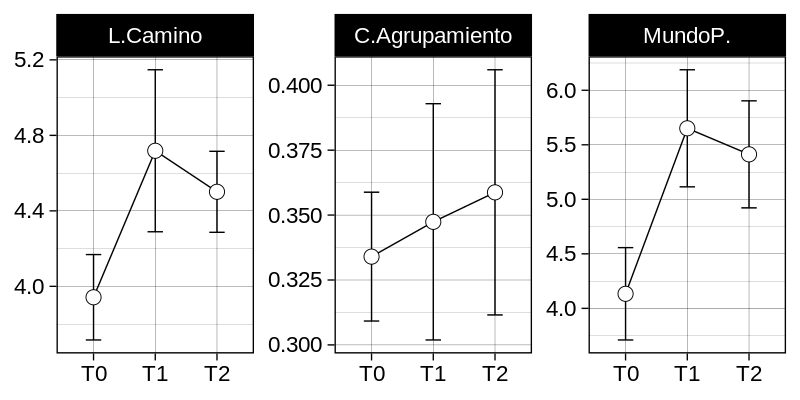
\includegraphics[width=0.9\textwidth]{graphL13.png}
    \caption{Métricas de mundo pequeño de pacientes con adicción en fase basal (T0), después de dos semanas tratamiento (T1) y tres meses de mantenimiento (T2)}
    \label{fig:gpL13}
\end{figure}


% Table created by stargazer v.5.2.2 by Marek Hlavac, Harvard University. E-mail: hlavac at fas.harvard.edu
% Date and time: Fri, Sep 20, 2019 - 03:39:49 AM
\begin{table}[!htbp] \centering
    \small
  \caption{Modelos de efectos mixtos de métricas de mundo pequeño en fase abierta del proyecto (dos semanas de tratamiento; tres meses de mantenimiento) con medidas demográficas como covariantes}
  \label{tab:memL12}
\begin{tabular}{@{\extracolsep{5pt}}lccc}
\\[-1.8ex]\hline
\hline \\[-1.8ex]
 & \multicolumn{3}{c}{Variables dependientes} \\
\cline{2-4}
\\[-1.8ex] & L.Camino & C.Agrupamiento & MundoP. \\
\\[-1.8ex] & (1) & (2) & (3)\\
\hline \\[-1.8ex]
 Fase(T1) & 0.778$^{***}$ & 0.010 & 1.465$^{***}$ \\
  & (0.076) & (0.007) & (0.098) \\
  Fase(T2) & 0.563$^{***}$ & 0.021$^{***}$ & 1.219$^{***}$ \\
  & (0.081) & (0.008) & (0.105) \\
  VAS & 0.014 & 0.0005 & 0.004 \\
  & (0.013) & (0.001) & (0.017) \\
  BIS-11 & $-$0.003 & $-$0.0004 & $-$0.005 \\
  & (0.003) & (0.0003) & (0.003) \\
  Sexo(F) & 0.051 & $-$0.028 & $-$0.295 \\
  & (0.168) & (0.024) & (0.294) \\
  Edad & 0.016$^{*}$ & 0.003$^{**}$ & 0.035$^{**}$ \\
  & (0.009) & (0.001) & (0.016) \\
  Educación & 0.025 & 0.001 & $-$0.004 \\
  & (0.022) & (0.003) & (0.038) \\
  Constante & 3.127$^{***}$ & 0.247$^{***}$ & 3.212$^{***}$ \\
  & (0.464) & (0.065) & (0.793) \\
 \hline \\[-1.8ex]
Observaciones & 48 & 48 & 48 \\
Crit. Inf. Akaike & 51.414 & $-$126.502 & 78.670 \\
Crit. Inf. Bayesiano & 70.126 & $-$107.790 & 97.382 \\
\hline
\hline \\[-1.8ex]
\textit{Nota:}  & \multicolumn{3}{r}{$^{*}$p$<$0.1; $^{**}$p$<$0.05; $^{***}$p$<$0.01} \\
\end{tabular}
\end{table}

\section{Fase abierta (6 meses)}
\subsection{Clínica}
Para explorar los cambios a seis meses de mantenimiento limitamos la muestra solamente a los 11 sujetos que completaron todas las fases experimentales y mediciones clínicas. En la tabla 5.11 se reportan los puntajes clínicos para cada medición por fase: basal (T0); tratamiento a dos semanas (T1); mantenimiento a tres (T2) y a seis meses (T3).

\begin{table}[!hbp]
    \centering
    \small
    \caption{Mediciones clínicas longitudinales (Basales: T0; Tratamiento: T1; Mantenimiento a tres meses: T2; Mantenimiento a seis meses: T3)}
    \label{tab:cl3}
\begin{tabular}{lccccc}
\hline
 & T0 & T1 & T2 & T3 \\
 & (N=11) & (N=11) & (N=11) & (N=11) \\
\hline
VAS   &  4.9 ±  4.3 &  1.1 ±  2.8 &  0.4 ±  1.0 &  2.6 ±  3.6 \\
CCQG  & 205.1 ± 39.7 & 136.5 ± 53.1 & 125.5 ± 50.5 & 155.7 ± 67.2 \\
CCQN  & 169.0 ± 52.7 & 121.5 ± 52.1 & 113.1 ± 35.1 & 112.3 ± 36.1 \\
BIS11 & 71.9 ± 14.4 & 55.4 ± 16.2 & 53.2 ± 12.4 & 57.9 ± 17.3 \\
\hline
\end{tabular}
\end{table}

Al visualizar gráficamente los cambios clínicos longitudinales en estos 11 sujetos, pudimos notar que el puntaje tuvo un ligero aumento en la última medición en contraste con las anteriores en varias de las mediciones, aún manteniéndose por debajo del puntaje basal (Fig \ref{fig:clin3}). \par
En cuanto al \textit{craving}, los modelos de efectos mixtos demostraron una interacción entre la 3ra fase experimental y el grupo de puntaje basal en la escala visual análoga, donde los sujetos expresaron un incremento en \textit{craving} comparado a la medición anterior. Esta diferencia fue mayor en quienes habían empezado con un nivel basal bajo ($-8.078\ (1.93),\ p<0.01$). Encontramos la misma interacción en la versión \textit{Now} del CCQ, donde los que tenían un \textit{craving} inicial alto siguieron disminuyendo mientras que los del otro grupo expresaron un aumento en su puntaje ($-70.63\ (29.42),\ p<0.05$). La versión General mostró un empeoramiento similar en ambos grupos, por lo que la interacción fue no significativa ($-47.97\ (34.8),\ p>0.05$). \par
En la medición de impulsividad encontramos un patrón similar: una interacción significativa ($-20.53\ (9.84),\ p<0.05$) donde mientras que el grupo de puntaje basal alto se mantuvo en niveles similares a la medición anterior el grupo de puntaje bajo demostró un incremento en sus niveles de impulsividad volviendo a niveles similares a los anteriores al tratamiento (tabla \ref{tab:clin3}).

\begin{figure}[!htb]
    \centering
    \begin{subfigure}[t]{0.475\textwidth}
        \centering
        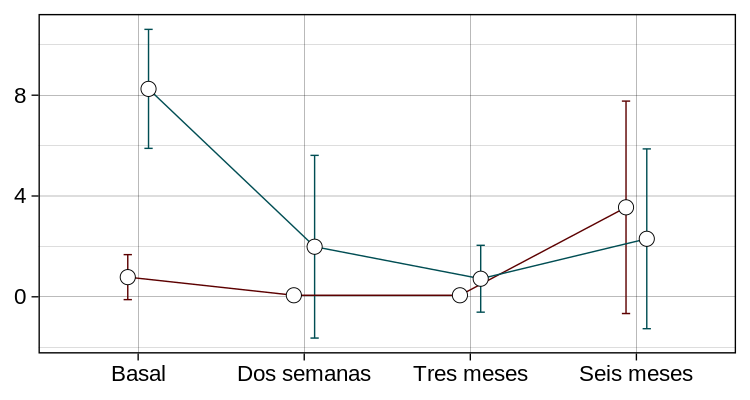
\includegraphics[width=\textwidth]{clinL21.png}
        \caption{VAS}
        \label{fig:cl3VAS}
    \end{subfigure}
    \hfill
    \begin{subfigure}[t]{0.475\textwidth}
        \centering
        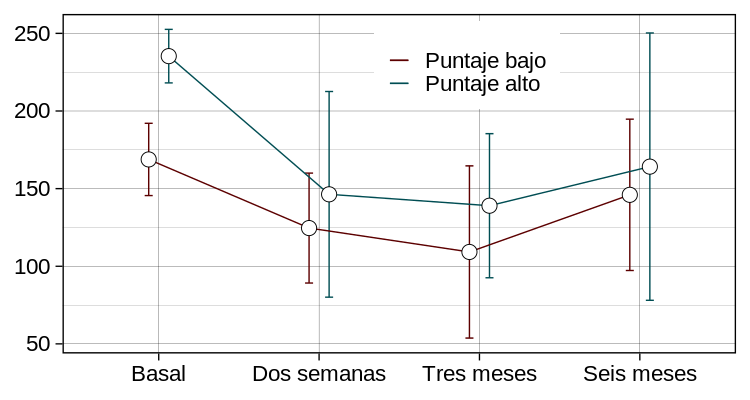
\includegraphics[width=\textwidth]{clinL22.png}
        \caption{CCQ-G}
        \label{fig:cl3CG}
    \end{subfigure}
    \vskip\baselineskip
    \begin{subfigure}[t]{0.475\textwidth}
        \centering
        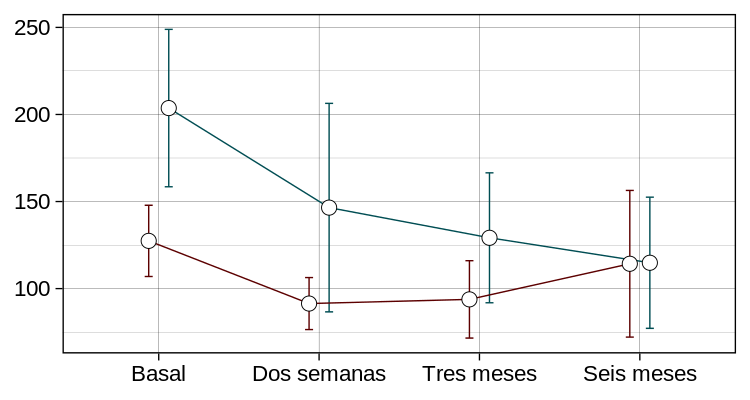
\includegraphics[width=\textwidth]{clinL23.png}
        \caption{CCQ-N}
        \label{fig:cl3CN}
    \end{subfigure}
    \hfill
    \begin{subfigure}[t]{0.475\textwidth}
        \centering
        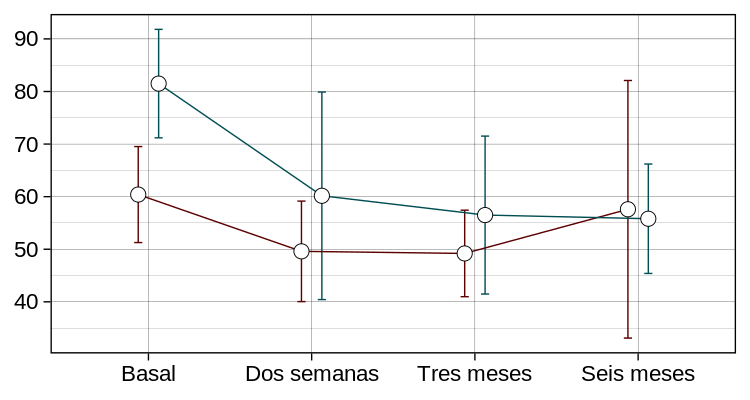
\includegraphics[width=\textwidth]{clinL24.png}
        \caption{BIS-11}
        \label{fig:cl3B11}
    \end{subfigure}
    \caption{Puntajes de mediciones clínicas basales, a dos semanas de tratamiento, tres y seis meses de mantenimiento separados por la mediana basal grupal}
    \label{fig:clin3}
\end{figure}

% Table created by stargazer v.5.2.2 by Marek Hlavac, Harvard University. E-mail: hlavac at fas.harvard.edu
% Date and time: Fri, Oct 18, 2019 - 12:00:39 PM
\begin{table}[!htbp] \centering
    \small
  \caption{Modelos de efectos mixtos de mediciones longitudinales (basales, dos semanas de tratamiento, tres meses y seis meses de mantenimiento) con grupo de puntaje basal y medidas demográficas como covariantes.}
  \label{tab:clin3}
\begin{tabular}{@{\extracolsep{5pt}}lcccc}
\\[-1.8ex]\hline
\hline \\[-1.8ex]
 & \multicolumn{4}{c}{Mediciones clínicas } \\
\cline{2-5}
\\[-1.8ex] & VAS & CCQ-G & CCQ-N & BIS-11\\
\\[-1.8ex] & (1) & (2) & (3) & (4)\\
\hline \\[-1.8ex]
  Fase(T1) & $-$0.720 & $-$44.200$^{*}$ & $-$36.000$^{*}$ & $-$10.800 \\
  & (1.422) & (25.695) & (21.721) & (7.269) \\
  Fase(T2) & $-$0.720 & $-$59.600$^{**}$ & $-$33.600 & $-$11.200 \\
  & (1.422) & (25.695) & (21.721) & (7.269) \\
  Fase(T3) & 2.130 & $-$23.200 & $-$18.200 & $-$2.800 \\
  & (1.422) & (25.695) & (21.721) & (7.269) \\
  Grupo(Mediana) & 7.953$^{***}$ & 103.218$^{***}$ & 82.065$^{***}$ & 21.272$^{**}$ \\
  & (1.445) & (32.135) & (25.469) & (9.279) \\
  Edad & 0.106$^{**}$ & 3.329$^{**}$ & 0.696 & $-$0.206 \\
  & (0.050) & (1.380) & (1.002) & (0.421) \\
  Sexo(F) & 0.699 & 11.717 & $-$10.510 & $-$7.222 \\
  & (1.477) & (35.627) & (27.067) & (10.813) \\
  Educación & $-$0.249$^{*}$ & $-$5.823 & $-$4.351 & $-$1.994$^{*}$ \\
  & (0.140) & (3.667) & (2.840) & (1.100) \\
  FaseT1:GrupoMed\textgreater  & $-$5.543$^{***}$ & $-$44.800 & $-$21.167 & $-$10.533 \\
  & (1.925) & (34.791) & (29.410) & (9.843) \\
  FaseT2:GrupoMed\textgreater  & $-$6.813$^{***}$ & $-$36.733 & $-$40.900 & $-$13.800 \\
  & (1.925) & (34.791) & (29.410) & (9.843) \\
  FaseT3:GrupoMed\textgreater  & $-$8.078$^{***}$ & $-$47.967 & $-$70.633$^{**}$ & $-$20.533$^{**}$ \\
  & (1.925) & (34.791) & (29.410) & (9.843) \\

  Constante & $-$0.410 & 95.177 & 154.671$^{***}$ & 94.598$^{***}$ \\
  & (2.717) & (67.908) & (53.061) & (19.726) \\
 \hline \\[-1.8ex]
Observaciones & 44 & 44 & 44 & 44 \\
Crit. Inf. Akaike & 203.268 & 397.696 & 385.241 & 315.496 \\
Crit. Inf. Bayesiano & 226.463 & 420.891 & 408.436 & 338.690 \\
\hline
\hline \\[-1.8ex]
\textit{Nota:}  & \multicolumn{4}{r}{$^{*}$p$<$0.1; $^{**}$p$<$0.05; $^{***}$p$<$0.01} \\
\end{tabular}
\end{table}

\FloatBarrier
\subsection{Topología de redes}

Para la evaluación a los seis meses longitudinal, utilizamos una submuestra de únicamente los sujetos que completaron la segunda fase de mantenimiento y el mismo nivel de $\tau$ que en análisis anteriores.

A los seis meses de mantenimiento observamos una disminución significativa en comparación con los niveles basales en la densidad ($-0.013\ (0.002),\ p<0.01$) y fuerza de las conexiones ($-1.139\ (0.256),\ p<0.01$). La edad fue una covariante significativa para la densidad de la red en esta submuestra de 11 sujetos ($0.001\ (0.0004),\ p<0.01$) como se figura en la tabla \ref{tab:memL2}. \par
Los análisis post-hoc demostraron que las diferencias en densidad entre la medición de mantenimiento y el resto de las mediciones fueron significativas (T3-T1, $-0.005\ (0.002),\ Z=-2.98,\ p<0.05$; T3-T2, $-0.007\ (0.002),\ Z=-4.059,\ p<0.001$). Para la medición de fuerza, estas diferencias fueron no significativas (T3-T1, $-0.334\ (0.240),\ Z=-1.412,\ p>0.05$; T3-T2, $-0.514\ (0.247),\ Z=-2.081,\ p>0.05$).

\begin{figure}[!htb]
    \centering
    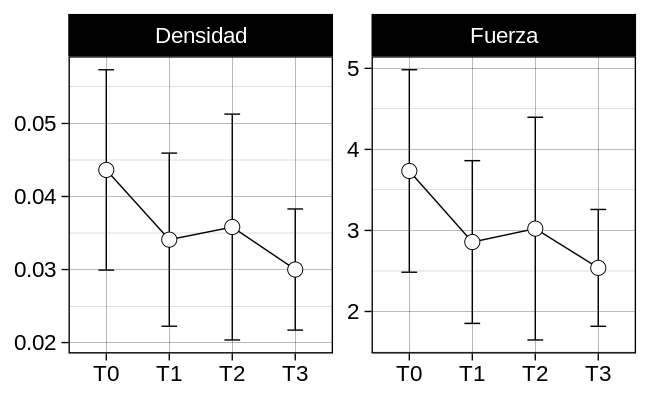
\includegraphics[width=0.7\textwidth]{graphL21.png}
    \caption{Medidas de densidad y fuerza de red en pacientes con adicción en mediciones basal (T0), a dos semanas de tratamiento (T1), tres meses (T2) y seis meses (T3) de mantenimiento}
    \label{fig:gpL21}
\end{figure}

En la eficiencia local hubo una diferencia significativa a los seis meses de mantenimiento en comparación con la medición basal ($-0.061\ (0.014),\ p<0.01$) encontrada en el modelo de efectos mixtos, y con el resto de las mediciones en los análisis post-hoc (T3-T1, $-0.039\ (0.013),\ Z=-2.97,\ p<0.05$; T3-T2, $-0.036\ (0.014),\ Z=-2.65,\ p<0.05$). Aunque en la eficiencia global hallamos una diferencia significativa entre la última medición post-mantenimiento y los niveles basales ($-0.059\ (0.008),\ p<0.01$), los análisis post-hoc no encontraron diferencias significativas de esta medición con el resto (T3-T1, $-0.01\ (0.007),\ Z=-1.516,\ p>0.05$; T3-T2, $-0.006\ (0.007),\ Z=-0.804,\ p>0.05$). Para ambas modalidades de eficiencia el sexo fue una covariante significativa en esta submuestra (eficiencia local, $-0.149\ (0.07),\ p<0.05$; eficiencia global, $-0.124\ (0.06),\ p<0.05$).

\begin{figure}[!htb]
    \centering
    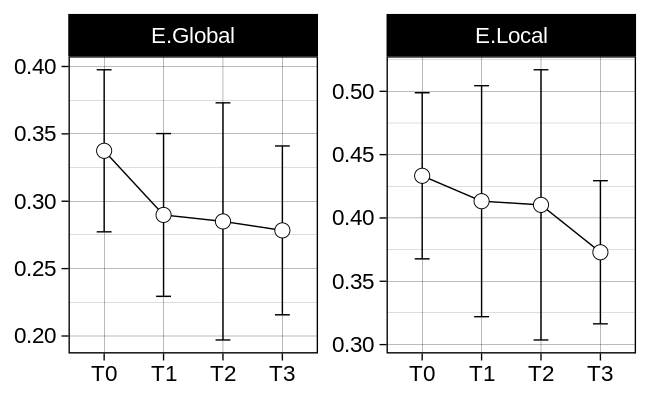
\includegraphics[width=0.7\textwidth]{graphL22.png}
    \caption{Medidas de eficiencia global y local de red en pacientes con adicción en mediciones basal (T0), a dos semanas de tratamiento (T1), tres meses (T2) y seis meses (T3) de mantenimiento}
    \label{fig:gpL22}
\end{figure}

% Table created by stargazer v.5.2.2 by Marek Hlavac, Harvard University. E-mail: hlavac at fas.harvard.edu
% Date and time: Fri, Oct 18, 2019 - 12:18:42 PM
\begin{table}[!htbp] \centering
    \small
  \caption{Modelos de efectos mixtos de medidas de topología de red en las mediciones longitudinales (basales, dos semanas de tratamiento, tres meses y seis meses de mantenimiento) con medidas clínicas y demográficas como covariantes}
  \label{tab:memL2}
\begin{tabular}{@{\extracolsep{5pt}}lcccc}
\\[-1.8ex]\hline
\hline \\[-1.8ex]
 & \multicolumn{4}{c}{Variables dependientes} \\
\cline{2-5}
\\[-1.8ex] & Densidad & Fuerza & E.Local & E.Global \\
\\[-1.8ex] & (1) & (2) & (3) & (4)\\
\hline \\[-1.8ex]
 Fase(T1) & $-$0.008$^{***}$ & $-$0.805$^{***}$ & $-$0.022 & $-$0.048$^{***}$ \\
  & (0.002) & (0.280) & (0.016) & (0.008) \\
  Fase(T2) & $-$0.007$^{***}$ & $-$0.630$^{**}$ & $-$0.025 & $-$0.053$^{***}$ \\
  & (0.002) & (0.297) & (0.016) & (0.009) \\
  Fase(T3) & $-$0.013$^{***}$ & $-$1.139$^{***}$ & $-$0.061$^{***}$ & $-$0.059$^{***}$ \\
  & (0.002) & (0.256) & (0.014) & (0.008) \\
  VAS & 0.00005 & 0.004 & $-$0.0004 & $-$0.0004 \\
  & (0.0002) & (0.033) & (0.002) & (0.001) \\
  BIS-11 & 0.0001 & 0.003 & 0.00001 & 0.0001 \\
  & (0.0001) & (0.008) & (0.0004) & (0.0002) \\
  Sexo(F) & $-$0.020$^{*}$ & $-$1.728$^{*}$ & $-$0.149$^{**}$ & $-$0.124$^{**}$ \\
  & (0.011) & (1.023) & (0.070) & (0.060) \\
  Edad & 0.001$^{**}$ & 0.059 & 0.005$^{**}$ & 0.005$^{**}$ \\
  & (0.0004) & (0.037) & (0.003) & (0.002) \\
  Educación & 0.001 & 0.043 & 0.003 & 0.003 \\
  & (0.001) & (0.104) & (0.007) & (0.006) \\
  Constante & 0.001 & 0.805 & 0.206 & 0.129 \\
  & (0.021) & (2.020) & (0.135) & (0.111) \\
 \hline \\[-1.8ex]
Observaciones & 44 & 44 & 44 & 44 \\
Crit. Inf. Akaike & $-$211.436 & 132.447 & $-$67.334 & $-$104.130 \\
Crit. Inf. Bayesiano & $-$191.810 & 152.074 & $-$47.708 & $-$84.504 \\
\hline
\hline \\[-1.8ex]
\textit{Nota:}  & \multicolumn{4}{r}{$^{*}$p$<$0.1; $^{**}$p$<$0.05; $^{***}$p$<$0.01} \\
\end{tabular}
\end{table}

En la longitud de camino característica encontramos un patrón de aumento constante desde la medición basal hasta los seis meses post-mantenimiento (T1, $0.443\ (0.054)$; T2, $0.41\ (0.057)$; T3, $0.530\ (0.049)$, todas $p<0.01$), mas ninguna de las mediciones post-hocs entre mediciones resultó significativa (T3\textendash{}T1, $0.083\ (0.046),\ Z=1.807,\ p>0.05$; T3\textendash{}T2, $0.116\ (0.047),\ Z=2.445,\ p>0.05$). Tanto sexo ($1.06l\ (0.544),\ p<0.05$) como edad ($-0.042 (0.019),\ p<0.05$) fueron covariantes significativas para esta métrica topológica. En esta submuestra no se encontraron cambios significativos en el coeficiente de agrupamiento entre las fases de medición, pero si una diferencia relativa al sexo ($-0.036\ (0.016),\ p<0.05$) (tabla \ref{tab:memL22}).\par
En la métrica de mundo pequeño observamos un aumento a los seis meses de mantenimiento ($0.827\ (0.149),\ p<0.01$). Los análisis post-hoc, por su parte, no demostraron diferencias significativas con la sesion post-tratamiento ($-0.24\ (0.132),\ Z=-1.81,\ p>0.05$) ni a los 3 meses de mantenimiento ($0.148\ (0.136),\ Z=1.09,\ p>0.05$).

\begin{figure}[!htb]
    \centering
    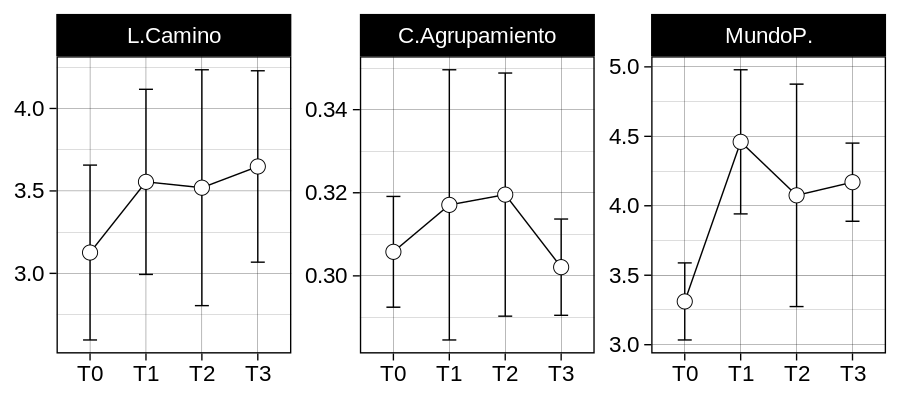
\includegraphics[width=0.9\textwidth]{graphL23.png}
    \caption{Métricas de mundo pequeño de pacientes con adicción en mediciones basal (T0), a dos semanas de tratamiento (T1), tres meses (T2) y seis meses (T3) de mantenimiento}
    \label{fig:gpL23}
\end{figure}

% Table created by stargazer v.5.2.2 by Marek Hlavac, Harvard University. E-mail: hlavac at fas.harvard.edu
% Date and time: Fri, Oct 18, 2019 - 12:23:01 PM
\begin{table}[!htbp] \centering
    \small
  \caption{Modelos de efectos mixtos de métricas de pequeño mundo en las mediciones longitudinales (basales, dos semanas de tratamiento, tres meses y seis meses de mantenimiento) con medidas clínicas y demográficas como covariantes.}
  \label{tab:memL22}
\begin{tabular}{@{\extracolsep{5pt}}lccc}
\\[-1.8ex]\hline
\hline \\[-1.8ex]
 & \multicolumn{3}{c}{Variables dependientes} \\
\cline{2-4}
\\[-1.8ex] & L.Camino & C.Agrupamiento & MundoP. \\
\\[-1.8ex] & (1) & (2) & (3)\\
\hline \\[-1.8ex]
 Fase(T1) & 0.443$^{***}$ & 0.006 & 1.117$^{***}$ \\
  & (0.054) & (0.009) & (0.162) \\
  Fase(T2) & 0.410$^{***}$ & 0.008 & 0.728$^{***}$ \\
  & (0.057) & (0.010) & (0.172) \\
  Fase(T3) & 0.530$^{***}$ & $-$0.008 & 0.827$^{***}$ \\
  & (0.049) & (0.009) & (0.149) \\
  VAS & 0.004 & $-$0.0001 & 0.004 \\
  & (0.006) & (0.001) & (0.019) \\
  BIS-11 & $-$0.0001 & $-$0.0003 & $-$0.003 \\
  & (0.002) & (0.0003) & (0.005) \\
  Sexo(F) & 1.067$^{**}$ & $-$0.036$^{**}$ & 0.668 \\
  & (0.544) & (0.016) & (0.436) \\
  Edad & $-$0.042$^{**}$ & 0.001$^{*}$ & $-$0.030$^{*}$ \\
  & (0.019) & (0.001) & (0.016) \\
  Educación & $-$0.011 & $-$0.001 & $-$0.030 \\
  & (0.054) & (0.002) & (0.045) \\
  Constante & 4.763$^{***}$ & 0.299$^{***}$ & 4.971$^{***}$ \\
  & (0.997) & (0.039) & (0.915) \\
 \hline \\[-1.8ex]
Observaciones & 44 & 44 & 44 \\
Crit. Inf. Akaike & 30.801 & $-$113.643 & 90.574 \\
Crit. Inf. Bayesiano & 50.427 & $-$94.017 & 110.200 \\
\hline
\hline \\[-1.8ex]
\textit{Nota:}  & \multicolumn{3}{r}{$^{*}$p$<$0.1; $^{**}$p$<$0.05; $^{***}$p$<$0.01} \\
\end{tabular}
\end{table}


